\section{No-IIGO Simulation}
\label{sec:ResultsAndEval:no-iigo}

Creating a baseline for comparison opened up the opportunity for more novel simulations. This section details an experiment on the IIGO - specifically, the impact of \emph{not} running the IIGO for an entire simulation. The impact of doing so is quantified using the metrics described in Section~\ref{sec:Simulations:Metric}.
This experiment was conducted by arbitrarily setting the cost of each action in the IIGO so high that there would be insufficient resources in the Common Pool to fund any of the roles. All other game config parameters were kept constant. 

The simulation was run ten times to account for the inherent stochasticity within various aspects of the game and the agents. The following subsections report the somewhat surprising results observed before analysing further and drawing conclusions about the importance of the IIGO.

\subsection{Results of No-IIGO Simulations}
\label{subsec:ResultsAndEval:no-iigo:results}

The most striking trend across all ten simulations was the state of the Common Pool. Inspection of the obtained Resource-time graphs revealed that the Common Pool contained little to no resources (less than 20) by the end of each of the simulations. The outcomes of the simulations were also far less deterministic than in the Baseline case, with large variatians seen most noticably in Archipaelago Survivability (defined in Section~\ref{sec:Simulations:Metric}).
Two Resource-Time graphs from the simulations are presented in Figure~\ref{fig:ResultsAndEval:no_iigo_unpredictable} below as representative samples of the outcomes of the experiment.


\begin{figure}[h]
    \centering
    \subfigure[Third Simulation]{
      \centering
      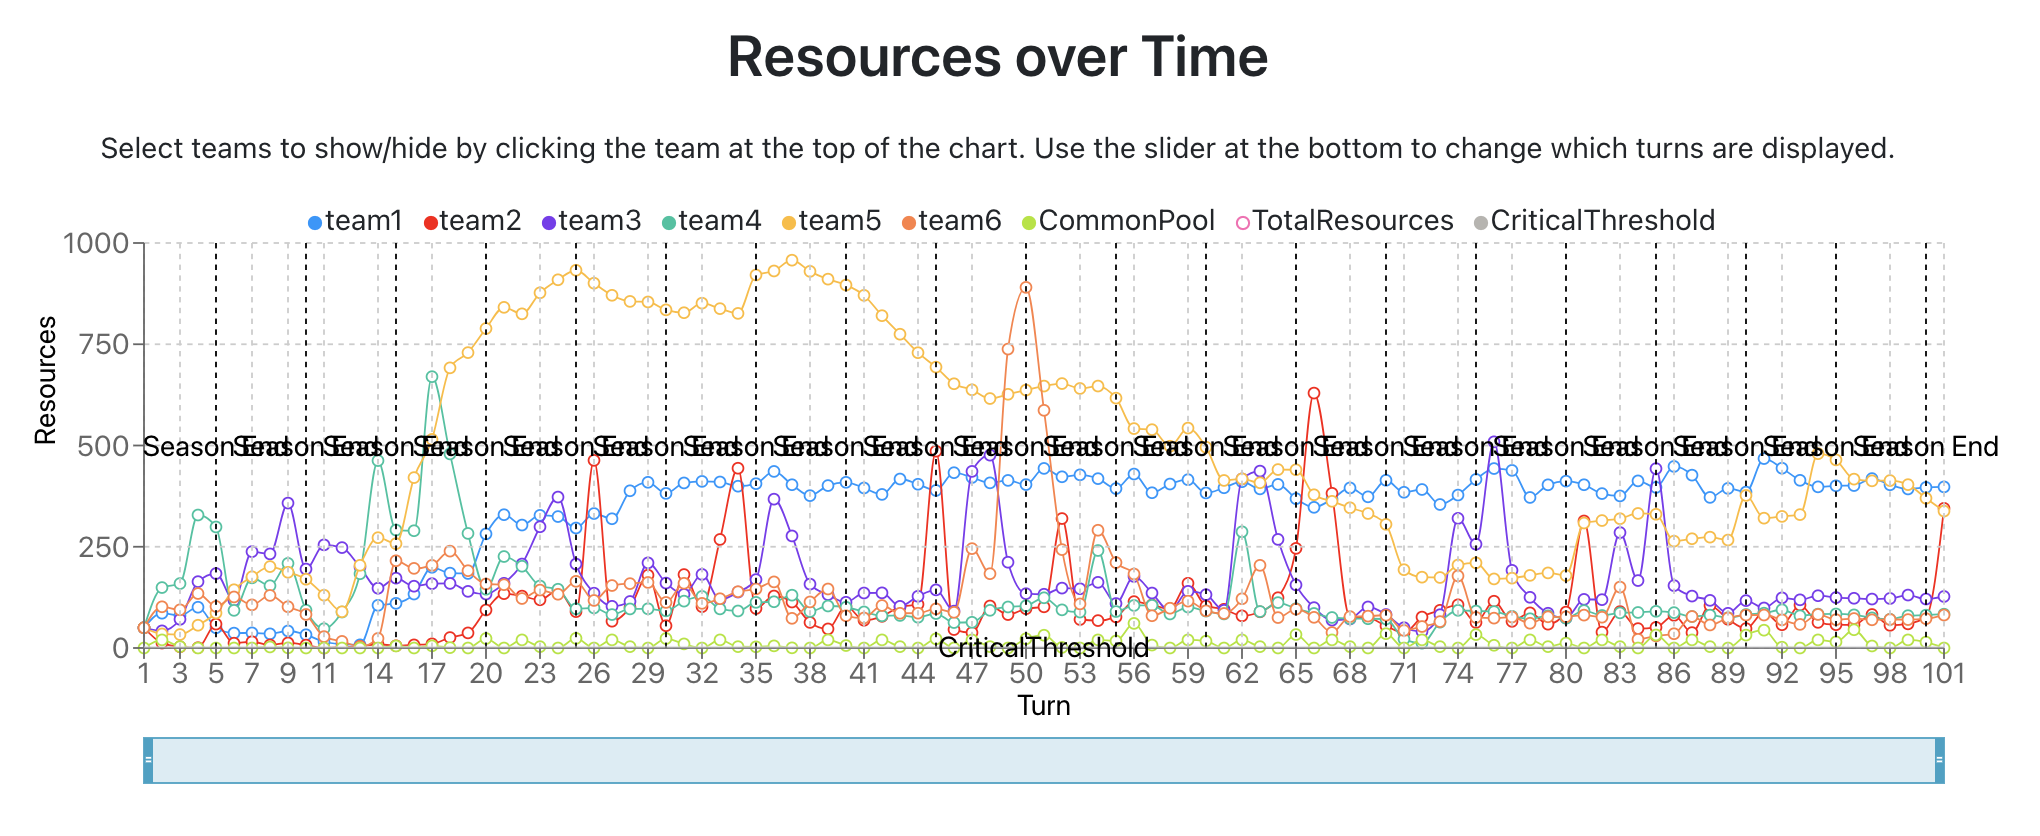
\includegraphics[width=.48\linewidth]{16_results_and_eval/images/no_iigo_1.png}
    }
    \subfigure[Sixth Simulation]{
      \centering
      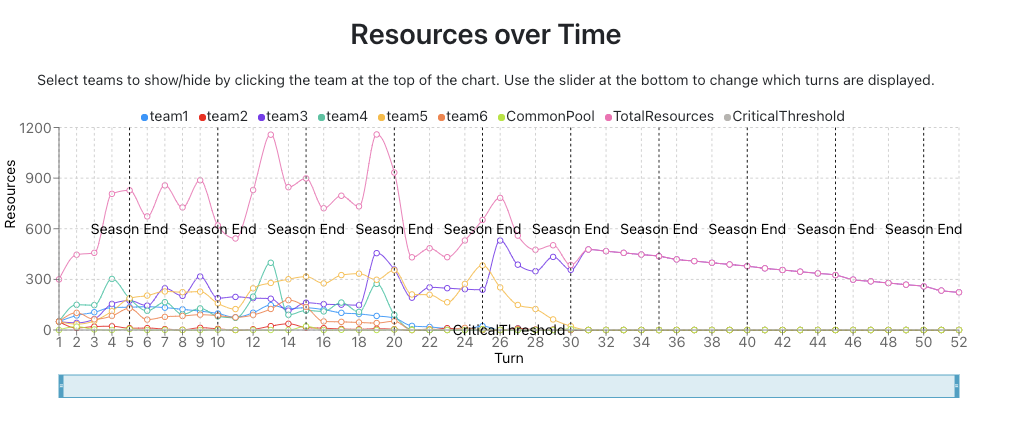
\includegraphics[width=.48\linewidth]{16_results_and_eval/images/no_iigo_2.png}
    }
    \caption{Unpredictability of outcomes in No-IIGO simulations}
    \label{fig:ResultsAndEval:no_iigo_unpredictable}
\end{figure}

Both simulations of the same experimental setup, Figures ~\ref{fig:ResultsAndEval:no_iigo_unpredictable}(a) and ~\ref{fig:ResultsAndEval:no_iigo_unpredictable}(b)) show a depleted Common Pool (light green line) with close to 0 resources throughout the entire simulation. While all agents were able to survive the full 100 turns in the former, only one was able to make it past the 30th turn in the latter, eventually dying at the 60th turn. 

The same metrics used to quantify the Baseline results in Table ~\ref{table:Simulations:num_metric} were monitored and aggregated for this experiment, as well as ten simulation of the Baseline configuration (with IIGO allowed to proceed at the usual cost). Table ~\ref{table:ResultsAndEval:iigo_vs_no_iigo} shows the results obtained:

\begin{table}[h]
    \centering
    \begin{tabular}{|l|c|c|c|c|}
    \hline
    \textbf{Metric}                     & \multicolumn{2}{c}{\textbf{Mean}}    & \multicolumn{2}{c}{\textbf{Standard Deviation}}   \\ \hline
                                        & \textbf{IIGO}      & \textbf{No IIGO}      &\textbf{IIGO}       & \textbf{No IIGO}                 \\ 
    \textbf{Archipelago Survivability}  & 100 & 93 & 0 & 16.36     \\
    \textbf{First Island Death}         & 100 & 55.2 & 0 & 42.64    \\
    \textbf{Gini Index}                 & 0.39 & 0.59 & 0.024 & 0.11   \\
    \textbf{Disasters Survived}         & 20 & 18.4 & 0 & 3.66    \\
    \textbf{ADDM}                       & 332.7 & 86.4 & 81.77 & 48.27    \\
    \textbf{AFS}                        & 1.91 & 1.57 & 0.11 & 0.17    \\ \hline
\end{tabular}
\caption{Metrics across ten simulations, with and without IIGO}
\label{table:ResultsAndEval:iigo_vs_no_iigo}
\end{table}


\subsection{Analysis of No-IIGO Simulation Results}
\label{subsec:ResultsAndEval:no-iigo:analysis_non_iigo_results}

\subsubsection{Comparison of Means}
\label{subsec:ResultsAndEval:no-iigo:comparison_of_means}
Comparing the means of the computed metrics shows a clear deterioration in performance of the agents when the IIGO does not run for the entire simulation. 
On average, an agent dies halfway through the simulation (turn 55) and the archipelago is unable to survive past 93 turns. 

Wealth is also far less equally distributed; the Average Gini Index is 50\% higher for the simulations without the IIGO. This can be attributed to the shorter lifespan of poorer islands, and the absence of the proportional tax system that is typically implemented in IIGO sessions. 

The removal of the IIGO also highlights the relationship between the long-term Collective Risk Dilemma (ltCRD) and the Foraging Dilemma. Without taxation, the Common Pool loses its most significant source of income. 
Without the IIGO, an island only contributes to the Common Pool when it believe a disaster is imminent. However, this contribution is entirely discretionary and at the mercy of the island's disaster prediction ability -- consequently, the Common Pool is often depleted (as per Figure~\ref{fig:ResultsAndEval:no_iigo_unpredictable}). 
Therefore, as the drastic reduction in the mean ADDM suggests, the burden of the cost of disasters falls on the islands. This also explains the reduction in the mean number of disasters survived by the archipelago. Islands with fewer resources are less likely to make optimal foraging decisions, resulting in the significant 17.8\% reduction in mean AFS shown in Table~\ref{table:ResultsAndEval:iigo_vs_no_iigo}.

The analysis shows that, paradoxically, parting with some resources in the form of taxation allows islands to make better investment decisions while foraging. Without the safety net of the Common Pool, the inability of the archipelago to address the ltCRD also affects its ability to address the Foraging Dilemma.


\subsubsection{Comparison of Standard Deviations}
\label{subsec:ResultsAndEval:no-iigo:comparison_of_std_devs}
Table~\ref{table:ResultsAndEval:iigo_vs_no_iigo} also shows a marked increase in the standard deviations of all the metrics used, with the exception of the ADDM. However, this can be attributed to the nearly four-fold reduction in its mean; expressing the standard deviation as a fraction of the mean shows that the uncertainty in the value of the ADDM increases more than two-fold without the IIGO.
The increase in uncertainty of all the metrics is supported by Figure ~\ref{fig:ResultsAndEval:no_iigo_unpredictable}, which provides a visual representation of how two simulations of the same experiment can have vastly different outcomes. 
These results reinforce the idea of the sensitivity of the agents to stochasticity, both within in the game environment (where the returns of foraging and damages from disasters are variable) and within the agents themselves (who, purely out of self-interest, may lie to each other during gift-exchange).


\subsection{Conclusion: Importance of the IIGO}
\label{subsec:Simulations:no-iigo:conclusion}

The above analysis shows that not only does the IIGO improve the performance of the archipelago across all the metrics of interest, it also acts as a stabilizing force in the game, making it far more deterministic. 
The main benefit of the IIGO is the taxation and allocation system it provides. By ensuring a stable, significant amount of resources in the Common Pool, this system provides damage mitigation against disasters, leaving agents with more resources for foraging. 
It also serves as a safety net for islands that are falling into the critical threshold, extending their lifespan and reducing the Gini Index of the archipelago.

While the IIGO might be a somewhat simplified implementation of modern governmental systems, the benefits it brings to the simulation are undeniable.
